\documentclass[a4paper,12pt,twoside]{memoir}

% Castellano
\usepackage[spanish,es-tabla]{babel}
\selectlanguage{spanish}
\usepackage[utf8]{inputenc}
\usepackage[T1]{fontenc}
\usepackage{lmodern} % scalable font
\usepackage{microtype}
\usepackage{placeins}

\RequirePackage{booktabs}
\RequirePackage[table]{xcolor}
\RequirePackage{xtab}
\RequirePackage{multirow}

% Links
\PassOptionsToPackage{hyphens}{url}\usepackage[colorlinks]{hyperref}
\hypersetup{
	allcolors = {red}
}

% Moneda
\usepackage{eurosym}

% Ecuaciones
\usepackage{amsmath}

% Rutas de fichero / paquete
\newcommand{\ruta}[1]{{\sffamily #1}}

% Párrafos
\nonzeroparskip

% Huérfanas y viudas
\widowpenalty100000
\clubpenalty100000

% Evitar solapes en el header
\nouppercaseheads

% Imagenes
\usepackage{graphicx}
\newcommand{\imagen}[2]{
	\begin{figure}[!h]
		\centering
		\includegraphics[width=0.9\textwidth]{#1}
		\caption{#2}\label{fig:#1}
	\end{figure}
	\FloatBarrier
}

\newcommand{\imagenflotante}[2]{
	\begin{figure}%[!h]
		\centering
		\includegraphics[width=0.9\textwidth]{#1}
		\caption{#2}\label{fig:#1}
	\end{figure}
}



% El comando \figura nos permite insertar figuras comodamente, y utilizando
% siempre el mismo formato. Los parametros son:
% 1 -> Porcentaje del ancho de página que ocupará la figura (de 0 a 1)
% 2 --> Fichero de la imagen
% 3 --> Texto a pie de imagen
% 4 --> Etiqueta (label) para referencias
% 5 --> Opciones que queramos pasarle al \includegraphics
% 6 --> Opciones de posicionamiento a pasarle a \begin{figure}
\newcommand{\figuraConPosicion}[6]{%
  \setlength{\anchoFloat}{#1\textwidth}%
  \addtolength{\anchoFloat}{-4\fboxsep}%
  \setlength{\anchoFigura}{\anchoFloat}%
  \begin{figure}[#6]
    \begin{center}%
      \Ovalbox{%
        \begin{minipage}{\anchoFloat}%
          \begin{center}%
            \includegraphics[width=\anchoFigura,#5]{#2}%
            \caption{#3}%
            \label{#4}%
          \end{center}%
        \end{minipage}
      }%
    \end{center}%
  \end{figure}%
}

%
% Comando para incluir imágenes en formato apaisado (sin marco).
\newcommand{\figuraApaisadaSinMarco}[5]{%
  \begin{figure}%
    \begin{center}%
    \includegraphics[angle=90,height=#1\textheight,#5]{#2}%
    \caption{#3}%
    \label{#4}%
    \end{center}%
  \end{figure}%
}
% Para las tablas
\newcommand{\otoprule}{\midrule [\heavyrulewidth]}
%
% Nuevo comando para tablas pequeñas (menos de una página).
\newcommand{\tablaSmall}[5]{%
 \begin{table}
  \begin{center}
   \rowcolors {2}{gray!35}{}
   \begin{tabular}{#2}
    \toprule
    #4
    \otoprule
    #5
    \bottomrule
   \end{tabular}
   \caption{#1}
   \label{tabla:#3}
  \end{center}
 \end{table}
}

%
%Para el float H de tablaSmallSinColores
\usepackage{float}

%
% Nuevo comando para tablas pequeñas (menos de una página).
\newcommand{\tablaSmallSinColores}[5]{%
 \begin{table}[H]
  \begin{center}
   \begin{tabular}{#2}
    \toprule
    #4
    \otoprule
    #5
    \bottomrule
   \end{tabular}
   \caption{#1}
   \label{tabla:#3}
  \end{center}
 \end{table}
}

\newcommand{\tablaApaisadaSmall}[5]{%
\begin{landscape}
  \begin{table}
   \begin{center}
    \rowcolors {2}{gray!35}{}
    \begin{tabular}{#2}
     \toprule
     #4
     \otoprule
     #5
     \bottomrule
    \end{tabular}
    \caption{#1}
    \label{tabla:#3}
   \end{center}
  \end{table}
\end{landscape}
}

%
% Nuevo comando para tablas grandes con cabecera y filas alternas coloreadas en gris.
\newcommand{\tabla}[6]{%
  \begin{center}
    \tablefirsthead{
      \toprule
      #5
      \otoprule
    }
    \tablehead{
      \multicolumn{#3}{l}{\small\sl continúa desde la página anterior}\\
      \toprule
      #5
      \otoprule
    }
    \tabletail{
      \hline
      \multicolumn{#3}{r}{\small\sl continúa en la página siguiente}\\
    }
    \tablelasttail{
      \hline
    }
    \bottomcaption{#1}
    \rowcolors {2}{gray!35}{}
    \begin{xtabular}{#2}
      #6
      \bottomrule
    \end{xtabular}
    \label{tabla:#4}
  \end{center}
}

%
% Nuevo comando para tablas grandes con cabecera.
\newcommand{\tablaSinColores}[6]{%
  \begin{center}
    \tablefirsthead{
      \toprule
      #5
      \otoprule
    }
    \tablehead{
      \multicolumn{#3}{l}{\small\sl continúa desde la página anterior}\\
      \toprule
      #5
      \otoprule
    }
    \tabletail{
      \hline
      \multicolumn{#3}{r}{\small\sl continúa en la página siguiente}\\
    }
    \tablelasttail{
      \hline
    }
    \bottomcaption{#1}
    \begin{xtabular}{#2}
      #6
      \bottomrule
    \end{xtabular}
    \label{tabla:#4}
  \end{center}
}

%
% Nuevo comando para tablas grandes sin cabecera.
\newcommand{\tablaSinCabecera}[5]{%
  \begin{center}
    \tablefirsthead{
      \toprule
    }
    \tablehead{
      \multicolumn{#3}{l}{\small\sl continúa desde la página anterior}\\
      \hline
    }
    \tabletail{
      \hline
      \multicolumn{#3}{r}{\small\sl continúa en la página siguiente}\\
    }
    \tablelasttail{
      \hline
    }
    \bottomcaption{#1}
  \begin{xtabular}{#2}
    #5
   \bottomrule
  \end{xtabular}
  \label{tabla:#4}
  \end{center}
}



\definecolor{cgoLight}{HTML}{EEEEEE}
\definecolor{cgoExtralight}{HTML}{FFFFFF}

%
% Nuevo comando para tablas grandes sin cabecera.
\newcommand{\tablaSinCabeceraConBandas}[5]{%
  \begin{center}
    \tablefirsthead{
      \toprule
    }
    \tablehead{
      \multicolumn{#3}{l}{\small\sl continúa desde la página anterior}\\
      \hline
    }
    \tabletail{
      \hline
      \multicolumn{#3}{r}{\small\sl continúa en la página siguiente}\\
    }
    \tablelasttail{
      \hline
    }
    \bottomcaption{#1}
    \rowcolors[]{1}{cgoExtralight}{cgoLight}

  \begin{xtabular}{#2}
    #5
   \bottomrule
  \end{xtabular}
  \label{tabla:#4}
  \end{center}
}




\graphicspath{ {./img/} }

% Capítulos
\chapterstyle{bianchi}
\newcommand{\capitulo}[2]{
	\setcounter{chapter}{#1}
	\setcounter{section}{0}
	\setcounter{figure}{0}
	\setcounter{table}{0}
	\chapter*{#2}
	\addcontentsline{toc}{chapter}{#2}
	\markboth{#2}{#2}
}

% Apéndices
\renewcommand{\appendixname}{Apéndice}
\renewcommand*\cftappendixname{\appendixname}

\newcommand{\apendice}[1]{
	%\renewcommand{\thechapter}{A}
	\chapter{#1}
}

\renewcommand*\cftappendixname{\appendixname\ }

% Formato de portada
\makeatletter
\usepackage{xcolor}
\newcommand{\tutor}[1]{\def\@tutor{#1}}
\newcommand{\course}[1]{\def\@course{#1}}
\definecolor{cpardoBox}{HTML}{E6E6FF}
\def\maketitle{
  \null
  \thispagestyle{empty}
  % Cabecera ----------------
\noindent
\includegraphics[width=\textwidth]{cabecera}\vspace{1cm}%
  \vfill
  % Título proyecto y escudo informática ----------------
  \colorbox{cpardoBox}{%
    \begin{minipage}{.8\textwidth}
      \vspace{.5cm}\Large
      \begin{center}
      \textbf{TFG del Grado en Ingeniería Informática}\vspace{.6cm}\\
      \textbf{\LARGE\@title{}}
      \end{center}
      \vspace{.2cm}
    \end{minipage}

  }%
  \hfill\begin{minipage}{.20\textwidth}
    
\includegraphics[width=\textwidth]{escudoInfor}
  \end{minipage}
  \vfill
  % Datos de alumno, curso y tutores ------------------
  \begin{center}%
  {%
    \noindent\LARGE
    Presentado por \@author{}\\ 
    en Universidad de Burgos --- \@date{}\\
    Tutor: \@tutor{}\\
  }%
  \end{center}%
  \null
  \cleardoublepage
  }
\makeatother

\newcommand{\nombre}{Miriam Torres Calvo} %%% cambio de comando
\newcommand{\nombreTutor}{Bruno Baruque Zanón}
\newcommand{\titulo}{Aplicaciones de Visión Artificial en Dispositivos de Edge Computing}

% Datos de portada
\title{\titulo \\Documentación Técnica}
\author{\nombre}
\tutor{\nombreTutor}
\date{\today}

\begin{document}

\maketitle



\cleardoublepage



%%%%%%%%%%%%%%%%%%%%%%%%%%%%%%%%%%%%%%%%%%%%%%%%%%%%%%%%%%%%%%%%%%%%%%%%%%%%%%%%%%%%%%%%



\frontmatter


\clearpage

% Indices
\tableofcontents

\clearpage

\listoffigures

\clearpage

\listoftables

\clearpage

\mainmatter

\appendix

\apendice{Plan de Proyecto Software}

\section{Introducción}
En este apéndice se va a mostrar la planificación del proyecto, la cuál es la base sobre la crea el proyecto \textit{software}. Desde el punto de vista de la temporalidad y viabilidad. 
Siendo está una parte fundamental del proyecto, ya que permite visualizar el escenario en el que se desarrollará, de tal forma que podamos realizar una alineación estrategica de los elementos que deben de ser completados, con el objetivo de finalizarlo correctamente.

\section{Planificación temporal}
La planificación temporal se

\section{Estudio de viabilidad}
En esta sección se va a desarrollar el estudio de la viabilidad del proyecto, con el objetivo de disponer de una visión global de los posibles benficios en contraposición del csote que supone el desarrollo del proyecto.
El desarrolo de cualquier proyecto \textit{software} lleva consigo una serie de riesgos, entre los que destacan la experiencia del equipo desarrollador, el tamaño del proyecto, el tiempo del que se dispone para llevarlo a cabo..., influyendo todo ello en el resultado final del proyecto.

\subsection{Viabilidad económica}
El primer paso del estudio, consiste en calcular la viabilidad económica del proyetco, para ello se deben de reportar y analizar los costes/beneficios que habría supuesto el proyecto en España \footnote{Nos referimos a España ya que, es el país dónde tiene lugar el desarrollo, y por ello se tendrán en cuenta los valores económica de dicho país.}.

\subsubsection{Costes}
El llevar a acabo la realización de un proyecto de esta envergadura, posee una serie de costes, tanto fijos cómo variables, los cuáles se van a desglosar en \textit{hardware}, \textit{software}, \textit{personal}\dots

\textbf{Costes Hardware}
Para llevar a cabo el proyecto, es necesario contar con algún que otro sistema \textit{hardware}, el primero de ellos es un equipo portátil. Se utilizará un MSI GS63 Stealth 8RE, con un procesador Intel Core i7 (8ª generación) de 6 núcleos a 2.2 GHz, con 16 GB de memoria RAM y una tarjeta gráfica 1060 de 6 GB, el cuál posee un precio del mercado de 2200 €, se tiene en cuenta que el tiempo de vida útil del equipo se enceuntra en torno a los seis años, 
por ello, de cara a los cálculos se tendrá en cuenta el tiempo de vida útil del inmovilizado, es decir, tres años.

A su vez, se necesita una Raspberry Pi, para poder trabajar con la aplicación desde un dispositivo con una capacdad de computo muy inferior al equipo principal de trabajo, en este caso se contará con una Raspberry Pi 3B, la cuál cuenta con un procesador Broadcom BCM2837 con 4 núcleos a 1,2 GHz y 1 GB de memoria RAM, la cuál posee un precio de 38 € y teniendo en cuenta que la vida útil es de aproximádamente seis años.
De la misma forma que con el portátil, se usará el tiempo medio de inmoviliado, es decir, tres años.

La amortización para ambos equipos es distinta, pero el tiempo de uso es el mismo, de noviembre de 2021 a septiembre de 2022, ambos incluidos, por ende, diez meses. A continuación, se detallarán todos los costes hardware (Tabla \ref{tab:costesHardw})

\begin{table}[H]
    \centering
    \begin{tabular}{lrr}
        \toprule
        \textbf{Concepto} & \textbf{Coste (\officialeuro)} & \textbf{Coste Amortizado (\officialeuro)}\\
        \midrule
        MSI GS63 Stealth 8RE & 2.200 & 611,11\\
        Raspberry Pi 3B & 38 & 10,55 \\
        \midrule
        \textbf{Total} & 2.238 & 621.66 \\
        \bottomrule
    \end{tabular}
    \caption{Costes de \emph{hardware}.}\label{tab:costesHardw}
\end{table}

\textbf{Costes Software}\\
Para el desarrollo del proyecto y uso del \textit{software} necesario, se necesita la adquisición de determinadas licencias, las cuáles se muestran a continuación , con su amortización correspondiente (Tabla \ref{tab:costesSoft}).

\begin{table}[H]
    \centering
    \begin{tabular}{lrr}
        \toprule
        \textbf{Concepto} & \textbf{Coste (\officialeuro)} & \textbf{Coste Amortizado (\officialeuro)}\\
        \midrule
        Fork & 49.99 & 41,66\\
        \TeX Works & 0 & 0 \\
        Windows 10 Pro & 259 & 215 \\
        Raspbian & 0 & 0 \\
        Visual Studio Code & 0 & 0 \\
        SonarCloud & 120 & 100 \\
        TensorFlow & 0 & 0 \\
        \midrule
        \textbf{Total} & 428,99 & 356.66 \\
        \bottomrule
    \end{tabular}
    \caption{Costes de \emph{software}.}\label{tab:costesSoft}
\end{table}

\textbf{Coste de personal}\\
El desarrollo del proyecto se ha llevado a cabo por un desarrollador y el tutor del proyecto.

\begin{itemize}
    \item El salario del desarrollador se calcula según~\cite{sueldoJunior}, siendo el salario medio anual del 20.201~\officialeuro{} netos al año.
    \item El salario del tutor se calcula según~\cite{sueldoInvest}, siendo el salario medio anual de 22.784~\officialeuro{} netos al año. Con una carga de trabajo de dos horas semanales.
\end{itemize}

La duración total del proyecto es de 40 semanas, por lo tanto el tutor trabajará un total de 80 horas, mientras que el desarrollador trabajará 800.

El IRPF es del 24\% y la retribución a la Seguridad Social, calculada tal cual se plantea en~\cite{ssCotizacion} por el Ministerio de Inclusión, Seguridad Social y Migraciones; se contribuye con un 31,40\% en total. Estando dividido en:
\begin{itemize}
    \tightlist
    \item 23,60\% de contingencias comunes~\cite{BOEPCM2442022}.
    \item 5,50\% por desempleo de tipo general~\cite{BOEPCM2442022}.
    \item 0,20\% destinado al Fondo de Garantía Salarial~\cite{BOEPCM2442022}.
    \item 0,60\% de formación profesional~\cite{BOEPCM2442022}.
    \item 1,50\% de tipo de cotización por accidentes de trabajo y enfermedades profesionales~\cite{BOEENFERMEDADES}.
\end{itemize}

\begin{table}[H]
    \centering
    \begin{tabular}{lrr}
        \toprule
        \textbf{Concepto} & \textbf{Desarrollador (\officialeuro)} & \textbf{Tutor (\officialeuro)}\\
        \midrule
        Salario total neto & 1.082,20 & 81 \\
        Retención IRPF & 259,73 & 19,44 \\
        Seguridad Social & 339,81 & 25,43 \\
        \midrule
        \textbf{Total salario bruto} &  1.681,74 & 125,87  \\
        \midrule
        \textbf{Total 10 meses} & 16.817,4 & 1.258,70 \\
        \bottomrule
    \end{tabular}
    \caption{Costes de personal.}\label{tab:costesPersonal}
\end{table}

En la Tabla \ref{tab:costesPersonal} se muestran de forma desgloasada los costes del personal, dando como coste final del personal:

16.817,40 \officialeuro (Desarrollador) + 1.258,70 \officialeuro (Tutor) = 18.076,10 \officialeuro

\textbf{Otros Costes}\\
Aqui se indican, costes que no son agrupables en ningún de los otros grupos, pero hay que tenerlos en cuenta.
Ver Tabla \ref{tab:costesOtros}

\begin{table}[H]
    \centering
    \begin{tabular}{lr}
        \toprule
        \textbf{Concepto (\officialeuro)} & \textbf{Coste (\officialeuro)} \\
        \midrule
        Logo & 20 \\
        Memoria impresa & 250 \\
        Alquiler oficina & 1600 \\
        Internet & 136\\
        Electricidad & 140 \\
        Agua & 51\\
        Calefacción & 230 \\
        \midrule
        \textbf{Total} & 2.427 \\
        \bottomrule
    \end{tabular}
\caption{Otros costes.}\label{tab:costesOtros}
\end{table}

A continaución, ver Tabla~\ref{tab:costesTotal}, se muestran los gastos totales del proyecto.

\begin{table}[H]
    \centering
    \begin{tabular}{lr}
        \toprule
        \textbf{Categoría (\officialeuro)} & \textbf{Coste (\officialeuro)} \\
        \midrule
        \textit{Hardware} & 2.238 \\
        \textit{Software} & 428,99 \\
        Personal & 18.076,10 \\
        Otros & 2.427 \\
        \midrule
        \textbf{Total} & 23.170,09 \\
        \bottomrule
    \end{tabular}
    \caption{Costes totales.}\label{tab:costesTotal}
\end{table}

\textbf{Beneficios}\\
De cara a la comercialización del proyecto, si se deseease obtener un beneficio económico del proyecto, se podría de manera sencilla crear un acceso por usuarios y que estos tengan diferentes niveles para acceder, número máximo de detecciones, número máximo de modelos que permite subir.
A su vez, también se podría plantear cómo un sistema de subscripción. En la Tabla \ref{tab:opcBen}

\begin{table}[H]
    \centering
    \begin{tabular}{lcrr}
        \toprule
        \textbf{Tipo} & \textbf{Detecciones} & \textbf{Modelos} & \textbf{Precio (\officialeuro)} \\
        \midrule
        \textit{Trial} & 5 & 2 & 0 \\
        \textit{Estudiante} & 25 & 5 & 10 \\
        \textit{Investigador} & 120 & 45 & 40 \\
        \textit{Equipo} & 300 & 100 & 150 \\
        \textit{Empresa} & Ilimitadas & 950 & 2000 \\
        \bottomrule
    \end{tabular}
    \caption{Posibles opciones para obtener beneficio del proyecto.}\label{tab:opcBen}
\end{table}

\textbf{Conclusiones}
Analizando los beneficios que se reportan en contraposición a los costes que conlleva el desarrollo del proyecto, queda demostrado su viabilidad. Se tiene ene cuenta, que el proyecto, no tiene la necesidad de ser mantenido, salvo por tener que añadir nuevos algoritmos de detección (y por ende, aceptar sus extensiones).


\subsection{Viabilidad legal}
En esta sección, principalmente se va a discutir el tema de la licencias, ya que al tratarse de un producto \textit{software} es la temática principal.

Según \cite{softwareLicense}, una licencia de \textit{software} es un contrato entre la entidad que ha creado y suministardo una aplicación, el código fuente de está o un producto relacionado con el mismo, y el usuario o usuarios finales.
La licencia es un documento, generalmente de texto, el cuál ha sido diseñado para proteger la propiedad intelectual del desarrollador del \textit{software} y para evitar reclamos en su contra debido a su uso.

Está, a su vez, proporciona, definiciones legalmente vinculantes para la definición y el uso del \textit{software}. Los derechos que posee el usuario final, también se encuentran detallados en la licencia.

\clearpage
\subsection{\textit{Software}}
La licencia más importante, es sobre la cuál se encuentra el \textit{software} desarrollado permitiendo así su uso.

El proyecto se encuentra licenciado bajo MIT. Ver Figura \ref{fig:license}.
\imagenflotante{license}{license}
\apendice{Especificación de Requisitos}

\section{Introducción}
En este apéndice se recogen las necesidades funcionales que deberán de ser soportadas por el sistema que va a ser desarrollado. Con el objetivo de obtener una buena documentación, deben de identificarse y describirse los requesitos que tienen que ser satisfacidos por el sistema, pero sin entrar en su proceso de realización.

\section{Objetivos generales}
Los objetivos del proyecto son los siguientes:
\begin{enumerate}
    \item Realización de una aplicación que permita la detección de objetos en diferentes tipos de represenatciones visuales y de diferentes formas.
    \item Creación de los \textit{datasets}, con los que se entrenarán los modelos y la obtención de estos en el formato, del algoritmo de detección usado.
    \item Creación/mejora de los diferentes scripts que permiten tanto la detección de los objetos, la conversión de formato de los modelos, la evaluación de \textit{accuracy} de lso diferentes modelos entrenados. 
    \item Conseguir que las interfaces a diseñar sean intuitivas y fáciles de utilizar. Deberán de ser transparentes al usuario, de tal forma, que se poseea un manejo de errores, ya sea producidos a nivel interno o por el usuario durante su uso.
    \item Permitir el uso de diferentes modelos asociados a la librería de Tensorflow.   
\end{enumerate}

\section{Catalogo de requisitos}
En esta sección se van a definir de forma clara y precisa todas las funcionalidades y restricciones del sistema.

\subsection{Requisitos funcionales}
\begin{itemize}
    \tightlist
    \item \textbf{RF-1 Uso de YOLOv4 como algoritmo de aprendizáje.} Se debe de ser capaz de entrenar un modelo mediante el algoritmo de detección de YOLOv4 y posteriormente utilizar dicho modelo para predecir sobre una representación visual.
    \begin{itemize}
    \tightlist
    \item \textbf{RF-1.1 Entrenar el modelo.} Se debe de poder entrenar tantos modelos como desee el usuario, los cuáles llevarán un periodo indefinido de tiempo, obteniendose en función de este mejores o peores resultados.
    \item \textbf{RF-1.2 Descarga del modelo.} Se debe de poder descargar/guardar el modelo, de cara a poder utilizarlo posteriormente.
    \item \textbf{RF-1.3 Conversion del modelo.} Se debe de poder convertir el modelo entrenado, el cuál posee un formato \textit{weights} a uno formato apto de la librería TensorFlow.
    \end{itemize}
    \item \textbf{RF-2 Detección de objetos}
    \begin{itemize}
      \tightlist
      \item \textbf{RF-2.1 Detección de objetos sobre una imagen.} Permitir el reconocimiento de los objetos que posee el modelo, a través de una imagen, guardar el resultado de la detección en un vídeo y un fichero CSV con las posiciones.
      \item \textbf{RF-2.2 Detección de objetos sobre un vídeo.} Permitir el reconocimiento de los objetos que posee el modelo, a través de una vídeo, guardar el resultado de la detección en un vídeo y un fichero CSV con las posiciones.
      \item \textbf{RF-2.3 Detección de objetos visualizados por la webcam.} Permitir el reconocimiento de los objetos que posee el modelo, a través de el vídeo que captura la webcam, guardar el resultado de la detección en un vídeo y un fichero CSV con las posiciones
      \item \textbf{RF-2.4 Contabilización de objetos sobre un vídeo.} Permitir la contabilización de los objetos que posee el modelo, a través de una vídeo, , guardar el resultado de la contabilización en un vídeo y un fichero CSV con las posiciones.
    \end{itemize}
\end{itemize}

\subsection{Requisitos no funcionales}
\begin{itemize}
\item \textbf{RNF-1 Usabilidad.} La plataforma debe de ser fácil tanto de aprender a utilizar como clara a la hora de reportar los errores que se puedan cometer. La interfaz debe ser intuitiva.
\item \textbf{RNF-2 Rendimiento.} La interfaz web debe de tener unos tiempos de carga razonables.
\item \textbf{RNF-3 Escalabilidad.} La plataforma debe soportar que se le añadan nuevas funcionalidades con relativa facilidad.
\item \textbf{RNF-4 Disponibilidad.} La plataforma debe de ser accesible a través de Internet sin importar la geolocalización del cliente.
\item \textbf{RNF-5 Mantenibilidad.} La plataforma debe cumplir los estándares de código de cada uno de los lenguajes en los que se desarrolla. 
\item \textbf{RNF-6 Soporte.} La plataforma debe dar soporte a ficheros CSV, MP4, JPG como mínimo. Así como ser compatible con HTML5.
\end{itemize}

\section{Especificación de requisitos}



\apendice{Especificación de diseño}

\section{Introducción}
En este apéndice se va a exponer cómo se han resuelto los objetivos anteriormente comentados. Así como la definición de datos que se utilizan en la aplicación, procedimientos ...

\section{Diseño de datos}
Al tratarse este proyecto de un proyecto de investigación, apenas cuenta con un diseño de datos. Por ello, se van a diferenciar los diferentes tipos de datos que componen la aplicación.
\begin{table}[H]
    \centering
    \begin{tabular}{l p{5cm}}
        \toprule
        \textbf{Objeto} & \textbf{Descripción}\\
        \midrule
        \textit{Modelo} & Elemento que permite la detección de los objetos para los cuáles ha sido entrenado. \\
        \textit{Fichero de etiquetas} & Clasifica la detecciones del objetos en fucnión de las posiciones el fichero. \\
        \textit{Resultados detección} & Imágenes, vídeos y ficheros CSV, que muestran la información obtenida tras la finalización de la detección. \\
        \bottomrule
    \end{tabular}
\end{table}

\section{Diseño procedimental}

En esta sección se recogen los detalles más relevantes en cuanto a los procedimientos llevados a cabo por la plataforma, según las acciones del usuario.

A continuación se explican lso diferentes diagrmas de secuencia (DS):

\begin{itemize}
    \item \textbf{DS para la subida del modelo.} Figura \ref{fig:subidaModeloCS}. Muestra el proceso que debe de seguir un usuario, para subir un modelo funcional y poder trabajar con él. Cuando el usuario se encuentra en la ventana modal correspondiente, deberá seleccionar el modelo que desea
    subir, si el fichero seleccionado, cumple con las validaciones del modelo, este se subirá, en caso contario, nos mostrará eñ mensaje de error concreto.
    \item \textbf{DS para la subida del fichero de etiquetas.} Figura \ref{fig:subidaEtiq}. Muestar el proceso que debe de seguir un usuario, para subir un fichero de etiquetas y poder trabajar con él. Cuando el usuario se encuentra en la ventana modal correspondiente, deberá seleccionar el fichero de etiquetas que desea
    subir, si el fichero seleccionado, cumple con las validaciones del fichero de etiquetas, este se subirá, en caso contario, nos mostrará eñ mensaje de error concreto.
    \item \textbf{DS para cambiar el modelo.} Figura \ref{fig:changeModelCS}. Muestra el proceso que debe de seguir un usuario, para cambiar el modelo actual por otro. Cuando el usuario se encuentra en la ventana modal correspondiente, deberá seleccionar el modelo deseado de la lista de los que se encuentran almacenados.
    \item \textbf{DS para cambiar el fichero de etiquetas.} Figura \ref{fig:changeEtiq}. Muestra el proceso que debe de seguir un usuario, para cambiar el fichero de etiquetas asignado en ese momento por otro. Cuando el usuario se encuentra en la ventana modal correspondiente, deberá seleccionar el fichero de etiquetas deseado de la lisat de todos los ficheros que se encuentran en el sistema.
    \item \textbf{DS para detectar objetos sobre un imagen.} Figura \ref{fig:imgDetect}. Muestra el procedimiento que debe de seguir un usuario para detectar los objetos del modelo, que se encuentran en la imagen, para ello una vez que el usuario se enecuentra en la ventana correspondiente deberá seleccionar la imagen que desea detectar, si todo va bien devolverá la imagen detectada, sino nos mostrar el mensaje de error.
    \item \textbf{DS para detectar objetos sobre un vídeo.} Figura \ref{fig:videoDetect}. Muestra el procedimiento que debe de seguir un usuario para detectar los objetos del modelo, que se encuentran en un vídeo, para ello una vez que el usuario se enecuentra en la ventana correspondiente deberá seleccionar el vídeo que desea detectar, si todo va bien devolverá el vídeo detectado, sino nos mostrar el mensaje de error. 
    \item \textbf{DS para la contabilziación de objetos.} Figura \ref{fig:OTVideo}. Muestra el procedimiento que debe de seguir un usuario para contabilizar los objetos del modelo, que se encuentran en un vídeo, para ello una vez que el usuario se enecuentra en la ventana correspondiente deberá seleccionar el vídeo que desea conyabilziar, si todo va bien devolverá el vídeo contabilzado, sino nos mostrar el mensaje de error.
    \item \textbf{DS para la detección de objetos a través de la webcam.} Figura \ref{fig:webcamDetect}. Muestra el procedimiento que debe de seguir un usuario para detectar los objetos del modelo, que se encuentran en a través de la webcam, para ello una vez que el usuario se enecuentra en la ventana correspondiente deberá decidir si solo deseea detectar o guardar el resultado de la detección, si todo va bien y se ha decidido guardar el resultado, este se devolverá como un vídeo, sino nos mostrar el mensaje de error.
    \item \textbf{DS para la detección de obejtos a través de la URL de la imagen.} Figura \ref{fig:urlDetect}. Muestra el procedimiento que debe de seguir un usuario para detectar los objetos del modelo, que se encuentran en la imagen que se lee a través de la URL, para ello una vez que el usuario se enecuentra en la ventana correspondiente deberá sintroducir la URL de la imagen que desea detectar, si todo va bien devolverá la imagen detectada, sino nos mostrar el mensaje de error.
    \item \textbf{DS para la detección de obejtos a través de la URL del vídeo de YouTube.} Figura \ref{fig:urlYTDetect}. Muestra el procedimiento que debe de seguir un usuario para detectar los objetos del modelo, que se encuentran en el vídeo de YouTube, para ello una vez que el usuario se enecuentra en la ventana correspondiente deberá introducir la URL del vídeo de YouTube qie deseea detectar, si todo va bien devolverá lel video detectado, sino nos mostrar el mensaje de error.
\end{itemize}

\imagen{subidaModeloCS}{Diagrama de Secuencia Subida Modelo de Detección}
\imagen{subidaEtiq}{Diagrama de Secuencia Subida Fichero de Etiquetas}
\imagen{changeModelCS}{Diagrama de Secuencia Cambio Modelo de Detección}
\imagen{changeEtiq}{Diagrama de Secuencia Cambio Fichero de Etiquetas}
\imagen{imgDetect}{Diagrama de Secuencia Detección Imagen}
\imagen{videoDetect}{Diagrama de Secuencia Detección Vídeo}
\imagen{OTVideo}{Diagrama de Secuencia Contabilización Vídeo}
\imagen{webcamDetect}{Diagrama de Secuencia Detección Webcam}
\imagen{urlDetect}{Diagrama de Secuencia Detección URL Imagen}
\imagen{urlYTDetect}{Diagrama de Secuencia Detección Vídeo YouTube}

\clearpage

\section{Diseño arquitectónico}
La estructura de la aplaicación es muy sencilla, ya que los modelos, ficheros de etiquetas y resultados de las detecciones se alamcenan en carpetas en el interior de la aplicación.
Guardándose de la siguiente manera:
\begin{table}[H]
    \centering
    \begin{tabular}{lr}
        \toprule
        \textbf{Objeto} & \textbf{Carpeta}\\
        \midrule
        \textit{Modelo} & checkpoints \\
        \textit{Fichero de etiquetas} & data\//classes \\
        \textit{Videos (URL)} & temp \\
        \textit{Resultados detección} & static\//detection \\
        \bottomrule
    \end{tabular}
    \caption{Carpetas donde se almacenan los fichero en la aplicación}
\end{table}
\apendice{Documentación técnica de programación}

\section{Introducción}
En este apéndice van a describirse de forma detallada la documentación técnica de programación. Se describirá la estructura de directorios que posee, la instalación y ejecución, así como las pruebas que se han llevado a cabo. 
\section{Estructura de directorios}
\begin{itemize}
    \tightlist
    \item \texttt{/}: es la raíz del proyecto dónde se encuentran tanto el README, la licencia y las carpetas contenedoras del código, documentación y las pruebas previas.
    \item \texttt{/codigo}: es la carpeta que contiene todo el código funcional del proyecto.
    \item \texttt{/codigo/checkpoints}: es la carpeta contenedora de los modelos de detección en formato Tensorflow, Tensorflow Lite y Tensor-RT.
    \item \texttt{/codigo/checkpoints/custom-416}: carpeta que contiene el modelo de detección de las matrículas, que posee el tamaño 416.
    \item \texttt{/codigo/checkpoints/custom-416/saved\_model.pb}: modelo en formato Tensorflow(.pb) de las matrículas.
    \item \texttt{/codigo/checkpoints/heads-416}: carpeta con el modelo de las cabezas en formato Tensorflow.
    \item \texttt{/codigo/checkpoints/heads-416/keras\_metadata.pb}: punto de control del modelo de conversión a .pb.
    \item \texttt{/codigo/checkpoints/heads-416/saved\_model.pb}: modelo detector de cabezas en formato Tensorflow(.pb)
    \item \texttt{/codigo/checkpoints/yolov4-416}: carpeta con el modelo oficial de YOLOv4 en formato Tensorflow.
    \item \texttt{/codigo/checkpoints/yolov4-416/keras\_metadata.pb}: punto de control del modelo de conversión a .pb.
    \item \texttt{/codigo/checkpoints/yolov4-416/saved\_model.pb}: modelo detector de YOLOv4 en formato Tensorflow(.pb)
    \item \texttt{/codigo/checkpoints/custom\_tfl-416}: carpeta con el modelo de detección de las matrículas en formato Tensorflow previo a la conversióna TensorFlow Lite.
    \item \texttt{/codigo/checkpoints/custom\_tfl-416/saved\_model.pb}: modelo detector de matrículas en formato Tensorflow(.pb) preparado para su conversión a .tflite.
    \item \texttt{/codigo/checkpoints/custom\_tflv2-416}: carpeta con el modelo de detección de las matrículas en formato Tensorflow previo a la conversióna TensorFlow Lite.
    \item \texttt{/codigo/checkpoints/custom\_tflv2-416/saved\_model.pb}: modelo detector de matrículas en formato Tensorflow(.pb) preparado para su conversión a .tflite.
    \item \texttt{/codigo/checkpoints/custom-416-int8.tflite}: modelo de detección de las matrículas en formato TensorFlow Lite(.tflite).
    \item \texttt{/codigo/checkpoints/custom-416v2.tflite.tflite}: modelo de detección de las matrículas en formato TensorFlow Lite(.tflite)
    \item \texttt{/codigo/checkpoints/models\_trt.txt}: fichero con los enlaces de los modelos de TensorRT.
    \item \texttt{/codigo/core}: carpeta con los ficheros de configuración utilizados durante el proyecto.
    \item \texttt{/codigo/core/backbone.py}: fichero de Python que contine las funciones relacionadas con la red YOLOv4
    \item \texttt{/codigo/core/commom.py}: fichero de Python que contine la clase BatchNormalization, para los ajustes de la red YOLOv4
    \item \texttt{/codigo/core/config.py}: fichero de Python que contine permite la selección de los ficheros de etiquetas de cara al uso del modelo
    \item \texttt{/codigo/core/functions.py}: fichero de Python que contine las funciones utilizadas en a lo largo de la detección de los objetos.
    \item \texttt{/codigo/core/utils.py}: fichero de Python que contine las funciones relacionadas con la red YOLOv4.
    \item \texttt{/codigo/core/yolov4.py}: fichero de Python que retorna el modelo de YOLO correspondiente.
    \item \texttt{/codigo/data}: carpeta que contine la información necesaria para la detección.
    \item \texttt{/codigo/data/anchors}: carpeta que contiene los anchors de lass diferentes redes.
    \item \texttt{/codigo/data/anchors/basline\_anchors.txt}: fichero de anchors.
    \item \texttt{/codigo/data/anchors/basline\_tiny\_anchors.txt}: fichero de anchors tiny.
    \item \texttt{/codigo/data/anchors/yolov3\_anchors.txt}: fichero de anchors yolov3.
    \item \texttt{/codigo/data/anchors/yolov3\_anchors.txt}: fichero de anchors yolov4.
    \item \texttt{/codigo/data/classes}: carpeta que contiene los fichero de etiquetas de los diferentes modelos.
    \item \texttt{/codigo/data/classes/coco.names}: fichero con las etiquetas del modelo oficial de YOLOV4.
    \item \texttt{/codigo/data/classes/custom.names}: fichero con las etiquetas del modelo de detección de matrículas.
    \item \texttt{/codigo/data/classes/heads.names}: fichero con las etiquetas del modelo de detección de las cabezas.
    \item \texttt{/codigo/data/classes/voc.names}: fichero de etiquetas del modelo de voc.
    \item \texttt{/codigo/data/classes/yymnist.names}: fichero de etiquetas del modelo de yymnist, detector de números.
    \item \texttt{/codigo/data/dataset}: carpeta que contiene los ficheros etiquetados a la hora de evaluar un modelo (ruta de la imagen posición detectada y valor de la clase).
    \item \texttt{/codigo/data/dataset/head.txt}: fichero de evaluacion del módelo de las cabezas. 
    \item \texttt{/codigo/data/dataset/license\_plate.txt}: fichero de evaluación del modelo de las matrículas.
    \item \texttt{/codigo/data/dataset/val2017.txt}: fichero de evaluación del modelo coco.
    \item \texttt{/codigo/data/images}: carpeta que contiene diferentes imagenes para su detección.
    \item \texttt{/codigo/data/video}: carpeta que contien diferentes vídeos para su detección/contabilización.
    \item \texttt{/codigo/deep\_sort}: carpeta que contiene los diferentes ficheros en Python para su evaluacion con Object Tracking.
    \item \texttt{/codigo/deep\_sort/detection.py}: fichero Python que contiene las funciones de detección para Obejct Tracking.
    \item \texttt{/codigo/deep\_sort/iou\_matching.py}: fichero Python que tiene las funciones de la maedida iou para Object Tracking.
    \item \texttt{/codigo/deep\_sort/kalman\_filter.py}: fichero Python que contiene el algoritmo del filtro de Kalman\cite{kalman_filter}.  
    \item \texttt{/codigo/deep\_sort/linear\_assignment.py}: Fichero Python que contiene las funciones relacionadas con la asignación linear.
    \item \texttt{/codigo/deep\_sort/nn\_matching.py}: Fichero Python con funciones de ajuste del algorimto de vecinos más cercanos\cite{knn}.
    \item \texttt{/codigo/deep\_sort/preprocessing.py}: Fichero Python con las funciones del preprocesado para Object Tracking.
    \item \texttt{/codigo/deep\_sort/track.py}: fichero Python que contiene las funciones necearias para detectar los objetos y sus etiquetas correspondeitnes, con su respectivo número de identificación.
    \item \texttt{/codigo/deep\_sort/tracker.py}: fichero Python que contiene las funciones necearias para detectar los objetos y sus etiquetas correspondeitnes, con su respectivo número de identificación.
    \item \texttt{/codigo/detections}: carpeta con el lso resultados de las detecciones obtenidas mediante la línea de comandos.
    \item \texttt{/codigo/detections/images}: carpeta con el resultado de las imagenes detectadas.
    \item \texttt{/codigo/detections/videos}: carpeta con el resultado de los vídeos detectados.
    \item \texttt{/codigo/mAP}: carpeta que contiene lso resultados de la evaluaciones de los modelos, así como scripts de ayuda para ello.
    \item \texttt{/codigo/mAP/extra}: carepeta con los cripts de ayuda para la evaluación del modelo.
    \item \texttt{/codigo/mAP/extra/intersect-gt-and-pred.py}: fichero Python que calcula la intersección entre la posición real del objeto y la obtenida por el modelo, con el objetivo de evaluar la calidad del modelo.
    \item \texttt{/codigo/mAP/extra/remove\_space.py}: fichero Python que elimina lso espacios de las etiquetas de las clases de los modelos.
    \item \texttt{/codigo/mAP/ground-truth}: carpeta que contiene los ficheros .txt de cada imagen a evalaur con sus posiciones originales en formato YOLO, junto el nombre de la etiqueta que le corresponde.
    \item \texttt{/codigo/mAP/predicted}: carpeta que contiene los ficheros .txt de cada imagen a evaluar con sus posiciones detectadas en formato YOLO, junto el nombre de la etiqueta que le corresponde.
    \item \texttt{/codigo/mAP/results\_custom\_tf\_complete}: carpeta con los resultados de la evalaución del modelo de las matrículas.
    \item \texttt{/codigo/mAP/results\_heads\_tf\_complete}: carpeta con los resultados de la evalaución del modelo de las cabezas.
    \item \texttt{/codigo/mAP/main.py}: fichero Python que representa el resultado de la evalaución del modelo.
    \item \texttt{/codigo/model\_data}: carpeta que contiene el modelo mars-small128.pb, utilizado en la inicialización de Obejct Tracking.
    \item \texttt{/codigo/static}: carpeta que contiene los ficheros 'estaticos' para Flask.
    \item \texttt{/codigo/static/css}: carpeta que contiene los diferentes ficheros de estilos\cite{css} usados a lo largo de la app Flask.
    \item \texttt{/codigo/static/js}: carpeta que contiene los diferentes scripts de JavaScript\cite{js} utilizados a lo largo de la app Flask.
    \item \texttt{/codigo/static/detections}: carpeta que contiene las imagenes, videos etiquetados tras su detección, así como los ficheros CSV de las posiciones.
    \item \texttt{/codigo/static/imgs}: carpeta con todas las imagenes usadas a lo largo de la app Flask.
    \item \texttt{/codigo/temp}: carpeta que almacena los ficheros de detección temporales, generados al inicio de las detecciones en la app Flask.
    \item \texttt{/codigo/templates}: carpeta que contienelos ficheros .html usados a lo alrgo de la app Flask.
    \item \texttt{/codigo/tools}: carpeta que contiene los scripts Python utilizados cómo herramientas a la hora de detectar.
    \item \texttt{/codigo/tools/freeze\_model.py}: script Python que convierte el gráfico del modelo de TensorFlow a uno con extensión .pb.
    \item \texttt{/codigo/tools/generate\_detections.py}: script Python que obtiene las 'cajas' en las cuáles se encuentran los objetos qu ehan sido detectados por el modelo.
    \item \texttt{/codigo/train}: carpeta que tiene los scripts de Python y de GoogleColab, así como los ficheros neecsarios para llevar a cabo el entrenamiento de un modelo de YOLOv4.
    \item \texttt{/codigo/trt}: carpeta que contiene el script de GoogleColab de conversión del fichero de pesos de YOLOv4 (.weights) a un modelo de TensorRT.
    \item \texttt{/codigo/app.py}: fichero de Python que es la propia app de Flask.
    \item \texttt{/codigo/convert\_tflite.py}: fichero de Python que convierte el modelo deseado a uno de TensorFlow Lite.
    \item \texttt{/codigo/convert\_trt.py}: fichero de Python que convierte el modelo deseado a uno de TensorRT.
    \item \texttt{/codigo/detect.py}: fichero de Python que detecta objetos en una imagen, según un modelo de detección.
    \item \texttt{/codigo/detectVideo.py}: fichero de Python que detecta objetos en una vídeo, según un modelo de detección.
    \item \texttt{/codigo/evaluate.py}: fichero de Python que evalua un modelo de detección, con el objetivo de medir su calidad a l hora de predeccir.
    \item \texttt{/codigo/objectTracker.py}: fichero de Python que contabiliza objetos en un vídeo, según un modelo de detección.
    \item \texttt{/codigo/preprocessDataEvaluate.py}: fichero de Python que obtiene las posiciones de las imágenes en el formato necesario apra su evalaución.
    \item \texttt{/codigo/save\_model\_tflite.py}: fichero de Python que convierte un fichero de pesos en formato .weights a un modelo de TensorFlow Lite. 
    \item \texttt{/codigo/save\_model.py}: fichero de Python que convierte un fichero de pesos en formato .weights a un modelo de TensorFlow.  
\end{itemize}

\section{Manual del programador}
En esta subsección se describen todos los recursos utilizados para poder llevar a cabo el proyecto.
De tal forma que un futuro desarrollador/mantenedor del proyecto no tenga inconvenientes a la hora de retomar el proyecto y conocerlo.

\subsection{Entorno de desarrollo}
Para poder continuar con el desarrollo del proyecto, será necesario contar con el siguiente \textit{software} instalado en el equipo:
\begin{itemize}
    \tightlist
    \item Python 3.7
    \item Bibliotecas de Python
    \item VSCode
\end{itemize}

A continuación, se comentára de forma detallada la instalación de los diferentes requerimientos.

\section{Compilación, instalación y ejecución del proyecto}

\section{Pruebas del sistema}

\apendice{Documentación de usuario}

\section{Introducción}
En este apendice se detallan los requerimientos de la aplicación, los pasos de instalación, despliegue, así como las indicaciones para su uso adecuado.
\section{Requisitos de usuarios}
Los requesitos para poder hacer uso de la aplicación son:
\begin{itemize}
    \item Tener instalado Python (minimo la version 3.7) y el resto de las librerías contenidas en el \textit{requeriments.txt}.
    \item Tener un navegador web compatible con HTML5 
\end{itemize}

\section{Instalación}
Instalar el contenedor docker de la aplicación.

\section{Manual del usuario}
En esta sección se explicarán las diferentes tareas que puede hacer un usario en la aplicación.
\imagen{homeAPP}{\textit{Home} de la aplicación}
\subsection{Carga de modelo de detección}
Esta opción se encuentra en el \textit{home} de la aplicación, correspondiendose esta opción con el primer botón, al hacer \textit{click} sobre él se nos abrirá una modal, la cuál cuenta con dos inputs, uno de tipo text y otro de tipo file(este posee funcionalidad de \textit{click} y de \textit{drag and drop}).
\begin{figure}[!h]
    \centering
    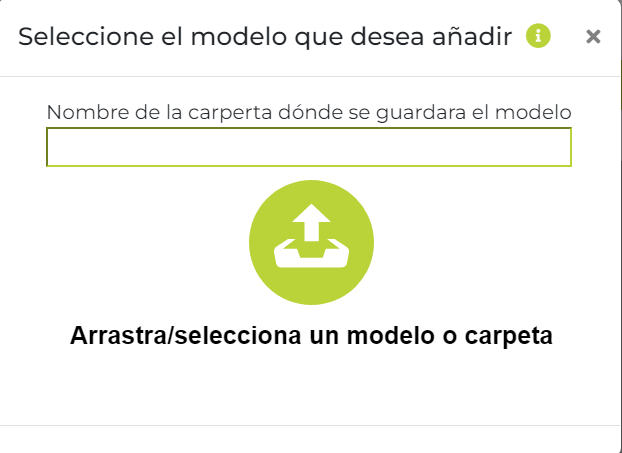
\includegraphics[width=0.6\textwidth]{modalModel}
    \caption{Modal para añadir modelos}\label{fig:modalModel}
\end{figure}
El input de tipo \textit{text}, sirve para introducir el nombre de la carpeta en la cuál se guardará el modelo de detección, de tal forma que sea más fácil encontrarlo posteriormente.
En segundo input de tipo \textit{file}, nos permite escoger el modelo que queremos añadir a la aplicación, ya sea un modelo de \textit{Tensorflow Lite} o una carpeta con el modelo de \textit{Tensorflow}.

\subsection{Carga de fichero de etiquetas}
Está opción se corresponde con el segundo botón de acciones del \textit{home}, al hacer \textit{click} sobre él se abrirá una modal, la cuál, es de un estilo similar a la modal de añadir modelos, en está encontraremos un input de tipo \textit{file}, el cuál funciona sólo por \textit{click}, el cuál permite la carga de archivos cuya extensión sea \textit{names}.
\begin{figure}[!h]
    \centering
    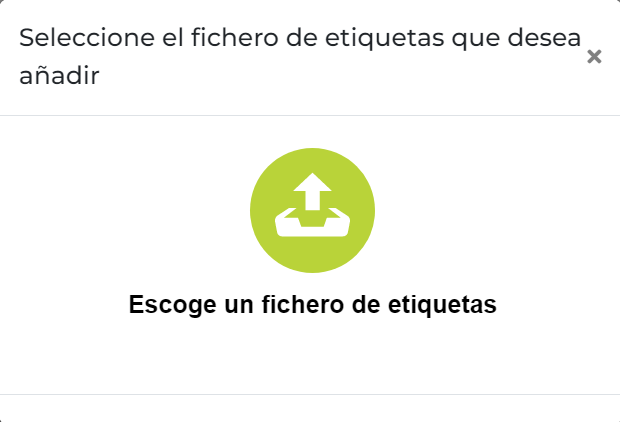
\includegraphics[width=0.6\textwidth]{modalNames}
    \caption{Modal para añadir ficheros de etiquetas}\label{fig:modalNames}
\end{figure}

\subsection{Cambiar fichero de etiquetas} \label{Cambiar fichero de etiquetas}
Esta opción, al igual que las dos anteriores, se encuentra en el \textit{home}, concretamente es el tercero de los botones de acciones, al hacer \textit{click} sobre él, se abrirá una ventana modal, la cuál posee el listado de todos los ficheros de etiquetas que posee la aplicación, encontrándose en cada acceso el fichero de etiquetas que se encuentra seleccionado (ver Imagen \ref{fig:modalNames}).
Para realizar un cambio de fichero, se debe de hacer \textit{click} en listado de los fichero, el cuál desplegara todos los los fichero que se encuentran en la aplicación, se selecciona el fichero con el que deseamos trabajar y hacemos \textit{click} en botón de \textbf{Cambiar fichero}.

\begin{figure}[!h]
    \centering
    
\includegraphics[width=0.6\textwidth]{selectNames}
    \caption{Modal para cambiar ficheros de etiquetas}\label{fig:selectNames}
\end{figure}

En el momento en el que se realice el cambio se mostrará el siguiente mensaje de confirmación (Ver Imagen: \ref{fig:OKSelectNames}) y tras su cierre se veremos como opción seleccionada el nuevo fichero de etiquetas.

\begin{figure}[!h]
    \centering
    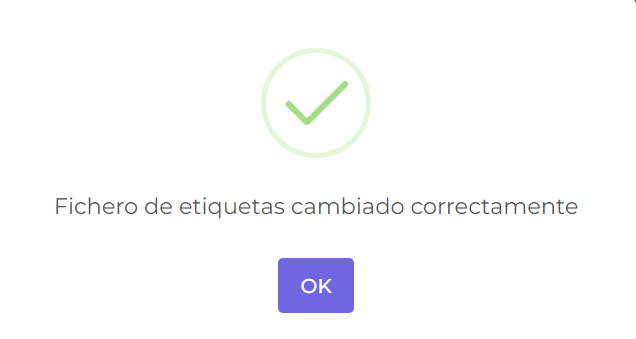
\includegraphics[width=0.6\textwidth]{OKSelectNames}
    \caption{Mensaje de confirmación de que el fichero de etiquetas se ha cambiado correctamente}\label{fig:OKSelectNames}
\end{figure}

\subsection{Cambiar modelo de detección}
Para llevar a cabo esta opción de la aplicación, se debe de hacer \textit{click} en el cuarto botón del listado de botones de acciones, el cuál abrirá una ventana modal, que contiene un menú de selección con todos los modelos que se encuentran en la aplicación(tanto modelos de Tensorflow(formato \textit{pb}) como modelos de Tensorflow Lite).

\begin{figure}[!h]
    \centering
    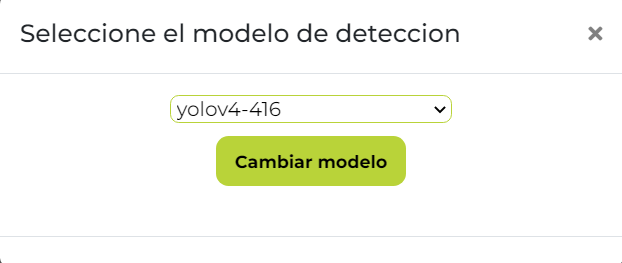
\includegraphics[width=0.6\textwidth]{selectModel}
    \caption{Modal para cambiar modelos de etiquetas}\label{fig:selectModel}
\end{figure}

La funcionalidad de esta modal es muy similar a la modal de \ref{Cambiar fichero de etiquetas}, en la cuál se encuentra seleccionado, al hacer \textit{click} sobre el listado de selección se mostrará todos los modelos que hay en la aplicación, para cambiar de modelo, tan sólo tendremos que cambiar el modelo seleccionado haciendo \textit{click} en la lista y escoger el modelo con el que deseamos trabajar.
El proceso del cambio tarda uno segundos, ya que, nos deja el modelo plenamente funcional para trabjar con él.

\subsection{Detección de objetos en una imagen} \label{od_img}
Esta opción se corresponde con la primera imagen de las seis que hay en el menú de detecciones.

\imagen{homeDetect}{Menú de detecciones}

Esta opción nos permite detectar objetos sobre una imagen, para ello debemos partir de un modelo y de un fichero de etiquetas seleccionado.
Al hacer \textit{click} sobre la imagen nos llevará a una nueva ventana, en la cuál podremos ver (al igual que en el homme), el modelo y el fichero de etiquetas seleccionado, 
a su vez, en la esquina superior izquierda un botón, <- volver al home, el cuál nos permite regresar al menú \textit{home}.

\imagen{odImg}{Página de detección de Objetos sobre una imagen}

Al hacer \textit{click} sobre el input, seleccionaremos la imagen la cuál deseamos etiquetar sus elementos, la cuál se nos mostrará en previsualización y nos "desbloqueará" un botón que nos permite detectar los objetos en la imagen.

\imagen{preDetectImg}{Imagen cargada para ser detectada}

Al hacer \textit{click} en \textbf{Detectar}, comenzará el proceso de detección y al acabar nos mostrará la imagen etiquetada, así como dos links de descarga(uno para la imagen etiquetada y otro para el fichero CSV de posiciones).

\imagen{posODImg}{Resultado de la detección en una imagen}

\subsection{Detección de objetos en un vídeo} \label{odVideo}
Esta opción se corresponde con la segunda de la opciones del menú de detecciones, la cuál nos permite detectar objetos sobre un vídeo.
Esta página posee los msimos datos informativos que la opción de \textbf{Detección de objetos en una imagen}(modelo de detección actual, modelo de detección actual y el botón de vuelta al home).

\imagen{odVideo}{Página de detección de Objetos sobre un vídeo}

La funcionalidad de esta opción es igual que la de detección en imagen (Ver \ref{od_img}), pero en lugar de seleccionar una imagen, se selecciona un vídeo.
El cuál, en cuanto se carga se previsualiza, permitiendonos reproducirlo. Al inicio de la detección, se nos mostrará el mensaje "Detectando... Si desea detener la detección pulse la tecla Q", de tal forma, que si deseamos parar la detección porque el vídeo es demasiado largo, 
o porque no nos interesá detectar todo el vídeo, podamos hacerlo y ver el resultado de la detección hasta ese punto. Al acabar la detección, podremos descargar el vídeo etiquetado y el fichero CSV de posiciones.

\begin{figure}[!h]
    \centering
    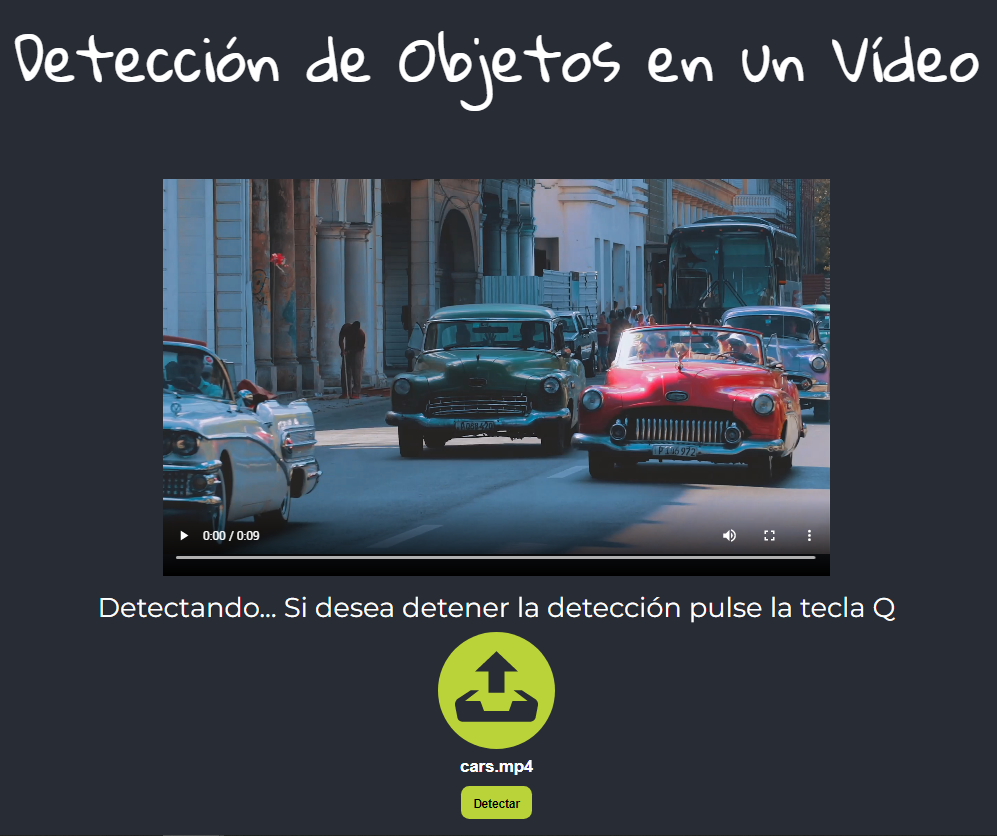
\includegraphics[width=0.6\textwidth]{stopOD}
    \caption{Proceso de detección de objetos en un vídeo}\label{fig:stopOD}
\end{figure}

\begin{figure}[!h]
    \centering
    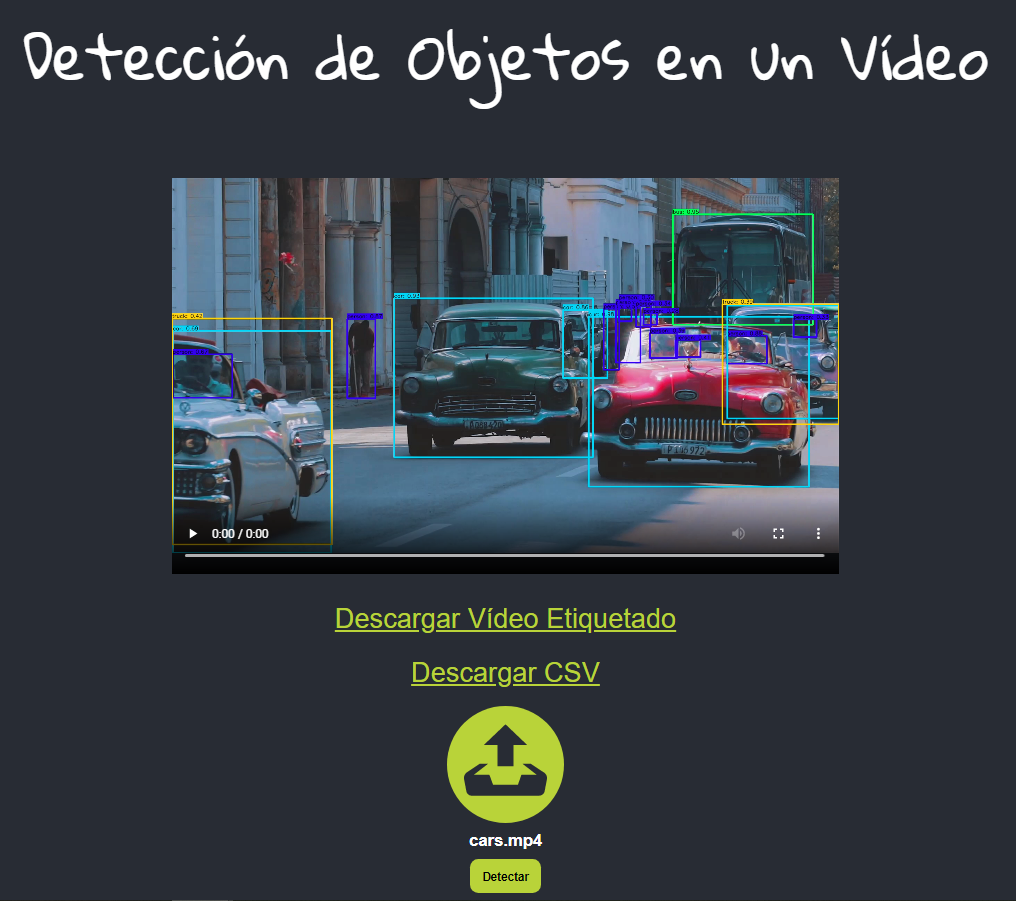
\includegraphics[width=0.6\textwidth]{odVideoEnd}
    \caption{Detección sobre vídeo teminada/detenida}\label{fig:odVideoEnd}
\end{figure}

\subsection{Contabilizar objetos en un vídeo} \label{odTrack}
Esta opción, se corresponde con la tercera opción del menú de detecciones, está funciona de la misma manera que \ref{odVideo}, deberemos seleccionar un vídeo en cuál se contabilizan los diferentes objetos que se encuentran en el vídeo.
Es decir, son dos opciones que s simple vista, funcioan exactamente igusl, pero realizan funciones de detección diferentes.

\subsection{Detección de objetos a tráves de la URL de una imagen} \label{odURl}
Esta opción es la cuarta de la lista de opciones de detección, la cuál nos permite detectar objetos sobre la url de una imagen, es decir, la detección se lleva a cabo sobre una imagen de Internet.

\imagen{odURL}{Detección de objetos sobre la URL de una imagen}

Para llevar a cabo la detección, deberemos de copiar la \textit{URL} de la imagen en el cuadro de texto, en el momento en el que el input detecte el contenid, nos mostrará el boton de \textbf{Detectar}.
Al hacer \textit{click} en el botón de \textbf{Detectar} comenzará el proceso de detección, lo cuál nos delvolverá un resultado correcto, siempre y cuándo la URL de la imagen poseea un \textit{.es} o un \textit{.com}.
Al acabar la detección, podremos descargar la imagen etiquetada y el fichero CSV de posiciones.

\imagen{odURLEnd}{Resultado de la detección a tráves de la URL de la imagen}

\subsection{Detección de objetos a tráves de la URL de un vídeo de YouTube}
Esta opción es la quinta del menú de detecciones, al igual que la función \ref{odURl} trabajan sobre las URLs de los objetos, pero esta trabaja sobre la \textit{url} de un vídeo de YouTube (es importante que esta url se obtenga desde la opción de compartir vídeo, y desde ahí copiar link, ya que de otra manera la detección nos daría error).
Al acabar la detección, podremos descargar el vídeo etiquetado y la fichero CSV de posiciones.

\imagen{odURL-YT}{Detección de objetos sobre la URL de un vídeo YouTube}

Al introducir la \textit{url}, dos mostrará el botón \textbf{Detectar} y al hacer \textit{click} sobre él, comezará el proceso de detección, al inicio de la detección
se nos mostrará el mensaje "Leyendo el vídeo de YouTube" ver imagen \ref{lvYT} y seguidamente "Detectando... Si desea detener la detección pulse la tecla Q", pudiendo detener la detección en cualquier momento, de la misma forma que en las opciones \ref{odVideo} y \ref{odTrack}.

\imagen{lvURL}{Leyendo el vídeo desde YouTube}
\imagen{resultOD-YT}{Resultado de la detección del vídeo de YouTube}

\subsection{Detección de objetos a tráves de webcam}
Esta opción es la última de las posibles opciones de detección, la cuál se encarga de detectar objetos a tráves de la \textit{webcam}, para esta opción es necesario poseer una cámara web.

\imagen{odWbcm}{Página de detección de objetos desde la Webcam}

Esta opción permite detectar objetos desde la \textit{webcam} sin que se grabe el vídeo, es decir, vemos el resultado en vivo pero no obtendremos, la opción de poder descargar el vídeo etiquetado, por otro lado, tendremos la opción de grabar el vídeo etiquetado para su posterior descarga.


\bibliographystyle{IEEEtran}
\bibliography{bibliografiaAnexos}

\end{document}
